\documentclass[10pt, xcolor=x11names, compress]{beamer}
%\documentclass[10pt, xcolor=x11names, compress, handout]{beamer}
\usetheme{progressbar}
%\usecolortheme[named=Purple4]{structure}
\progressbaroptions{headline=sections,titlepage=normal,frametitle=normal}

\setbeamertemplate{navigation symbols}{}

\usepackage{iwona} 

\usepackage{alltt}
\usepackage{amsmath,amsfonts, amssymb, amscd}
\usepackage{hyperref}
\usepackage{setspace}
\usepackage{wasysym}
\usepackage{ulem}

\usepackage{calc}
\usepackage[overlay,absolute]{textpos}
\TPGrid[5mm,5mm]{20}{20}



\renewcommand{\Re}{\operatorname{Re}}
\renewcommand{\Im}{\operatorname{Im}}
\newcommand{\debye}{\operatorname{debye}}

\newcommand{\chik}{$\chi(k)$}
\newcommand{\chir}{$|\tilde{\chi}(R)|$}


\newcommand{\file}[1]{{\color{Firebrick4}\texttt{`#1'}}}
\newcommand{\multiple}{{\color{Orange3}\textsl{multiple}}}


\newcommand{\atoms}  {{\color{DarkOrchid4}\textsc{atoms}}}
\newcommand{\feff}   {{\color{DarkOrchid4}\textsc{feff}}}
\newcommand{\ifeffit}{{\color{DarkOrchid4}\textsc{ifeffit}}}
\newcommand{\athena} {{\color{DarkOrchid4}\textsc{athena}}}
\newcommand{\artemis}{{\color{DarkOrchid4}\textsc{artemis}}}

\renewenvironment<>{center}
{\begin{actionenv}#1\begin{originalcenter}}
{\end{originalcenter}\end{actionenv}}

\definecolor{guessp}   {rgb}{0.64,0.00,0.64}
\newcommand{\guessp}   {{\color{guessp}guess}}
\definecolor{defp}     {rgb}{0.00,0.55,0.00}
\newcommand{\defp}     {{\color{defp}def}}
\definecolor{setp}     {rgb}{0,0,0}
\newcommand{\setp}     {{\color{setp}set}}
\definecolor{lguessp}  {rgb}{0.24,0.11,0.56}
\newcommand{\lguessp}  {{\color{lguessp}lguess}}
\definecolor{skipp}    {rgb}{0.70,0.70,0.70}
\newcommand{\skipp}    {{\color{skipp}skip}}
\definecolor{restrainp}{rgb}{0.80,0.61,0.11}
\newcommand{\restrainp}{{\color{restrainp}restrain}}
\definecolor{afterp}   {rgb}{0.29,0.44,0.55}
\newcommand{\afterp}   {{\color{afterp}after}}
\definecolor{penaltyp} {rgb}{0.55,0.35,0.17}
\newcommand{\penaltyp} {{\color{penaltyp}penalty}}
\definecolor{mergep}   {rgb}{0.93,0.00,0.00}
\newcommand{\mergep}   {{\color{mergep}merge}}


%% define new commands here
%\newcommand{\eto}{EuTiO$_3$}

\mode<presentation>

\title{Discussion of the Uranyl Hydrate EXAFS Analysis Example}
%\subtitle{}

\author{Bruce Ravel}
\institute[NIST]{Synchrotron Methods Group, Materials Measurement Science Division\\%
  Materials Measurement Laboratory\\%
  National Institute of Standards and Technology\\%
  \&\\%
  Local Contact, Beamline X23A2\\%
  National Synchrotron Light Source\\~}


\date[Diamond2011]{EXAFS Data Analysis workshop 2011\\
  Diamond Light Source\\November 14--17, 2011\\~}

%\date[Diamond2011]{EXAFS Data Analysis workshop 2011\\
%  Diamond Light Source\\November 14--17, 2011}

\begin{document}
\maketitle

\begin{frame}
  \frametitle{Copyright}
  \tiny

  This document is copyright \copyright 2007-2010 Bruce Ravel.

  \begin{center}
    
\includegraphics[width=1.0cm]{images/somerights20}
  \end{center}

  This work is licensed under the Creative Commons
  Attribution-ShareAlike License.  To view a copy of this license,
  visit \href{http://creativecommons.org/licenses/by-sa/3.0/}
  {\color{Purple4}\texttt{http://creativecommons.org/licenses/by-sa/3.0/}}
  or send a letter to Creative Commons, 559 Nathan Abbott Way,
  Stanford, California 94305, USA.

  \begin{description}
  \item[You are free:] %
    \begin{itemize}
    \item \textbf{to Share} --- to copy, distribute, and transmit the work
    \item \textbf{to Remix} --- to adapt the work
    \end{itemize}
  \item[Under the following conditions:] %
    \begin{itemize}
    \item Attribution. You must attribute the work in the manner
      specified by the author or licensor (but not in any way that
      suggests that they endorse you or your use of the work).
    \item Share Alike. If you alter, transform, or build upon this
      work, you may distribute the resulting work only under the same,
      similar or a compatible license.
    \item Any of these conditions can be waived if you get permission
      from the author.
    \end{itemize}
  \end{description}
  \begin{itemize}
  \item For any reuse or distribution, you must make clear to others
    the license terms of this work. The best way to do this is with a
    link to the URL for this document.
  \item Any of the above conditions can be waived if you get
    permission from the copyright holder.
  \item Nothing in this license impairs or restricts the author's
    moral rights.
  \end{itemize}

  Your fair dealing and other rights are in no way affected by the
  above.  This is a human-readable summary of the Legal Code (the full
  license).


\end{frame}

%%% Local Variables:
%%% mode: latex
%%% TeX-master: "pimst2"
%%% End:


\begin{frame}
  \frametitle{The sample}
  \begin{columns}[T]
    \begin{column}{0.5\linewidth}
      1000 ppm uranyl nitrate solution dissolved in DI water, pH=0.96\\[3ex]

      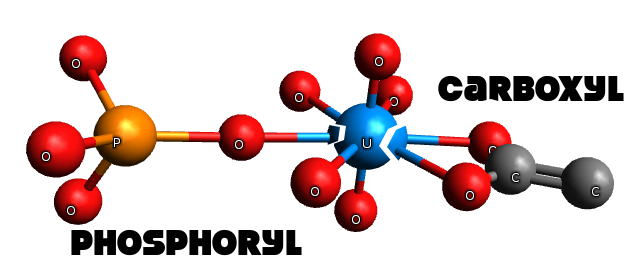
\includegraphics[width=\linewidth]{uranyl.pdf}

      \bigskip

      The liquid was held in a fluid cell and measured in fluorescence.
    \end{column}
    \begin{column}{0.5\linewidth}
      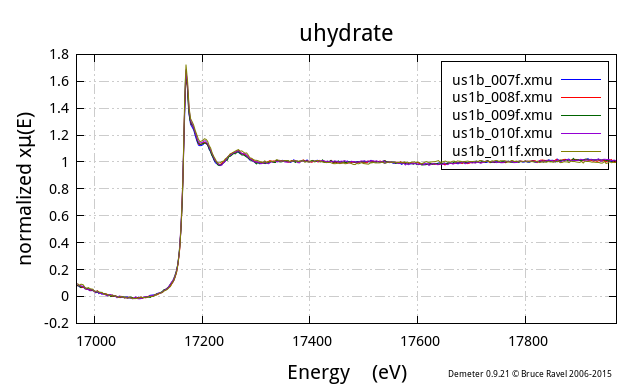
\includegraphics[width=\linewidth]{images/uhydrate_mu.png}

      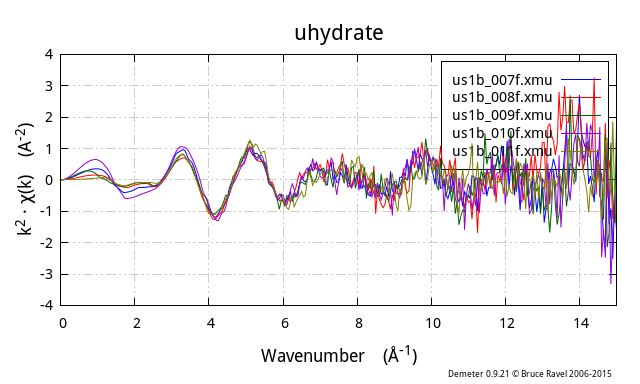
\includegraphics[width=\linewidth]{images/uhydrate_chi.png}
    \end{column}
  \end{columns}

  \begin{textblock*}{0.7\linewidth}(0pt,19.0\TPVertModule)%
    \tiny%
    S.D.\ Kelly, et al., \textit{X-ray absorption fine structure
      determination of pH-dependent U-bacterial cell wall
      interactions}, Geochimica et Cosmochimica Acta \textbf{66}:22
    (2002) pp\  3855-3871.
    \href{http://dx.doi.org/10.1016/S0016-7037(02)00947-X}
    {\color{Blue4}\texttt{DOI:10.1016/S0016-7037(02)00947-X}}
  \end{textblock*}
\end{frame}

\begin{frame}
  \frametitle{Statistical noise and systematic noise}
  \begin{columns}[T]
    \begin{column}{0.5\linewidth}
      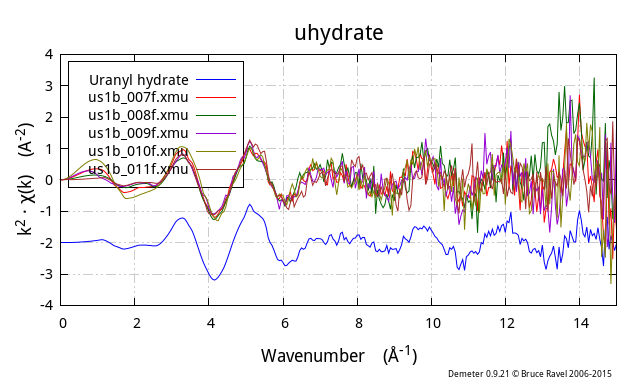
\includegraphics[width=\linewidth]{images/merged_chi.png}
      
    \end{column}
    \begin{column}{0.5\linewidth}
      \begin{tabular}{lr}
        data & \multicolumn{1}{c}{$\epsilon_k$} \\
        \hline
        5 scans & $\sim4.76\times10^{-3}$ \\
        merge   & $1.77\times10^{-3}$
      \end{tabular}
      $$\frac{\epsilon_1}{\epsilon_{merge}} = 2.69$$
      $$\sqrt{5} \approx 2.24$$
    \end{column}
  \end{columns}
  \begin{block}{The data seem show the behavior of statistcal noise}
    But is the signal at 14\,\AA$^{-1}$ really data?  In fact, is the
    signal beyond 9\,\AA$^{-1}$ really data?
  \end{block}
  \begin{alertblock}{}
    \centering In any case, how to we proceed with a molecule in solution?
  \end{alertblock}
\end{frame}

\begin{frame}[fragile]
  \frametitle{Sodium uranyl triacetate}
  \begin{columns}[T]
    \begin{column}{0.7\linewidth}
      Here's a crystal that contains the uranyl moiety:
      \begin{center}
        \begin{minipage}{0.75\linewidth}
          \begin{block}{}
            \tiny
            \begin{alltt}
{\color{Green4}title Na uranyl triacetate}
{\color{Green4}title Templeton, et al, Acta Cryst 1985 C41 1439-1441}
{\color{SteelBlue4}space} = P 21 3
{\color{SteelBlue4}rmax}  = 7.0    {\color{SteelBlue4}a}=10.689
{\color{SteelBlue4}core}  = U
{\color{Purple4}atoms}
{\color{Blue4}! At.type   x         y         z      tag}
  U        0.4294    0.4294    0.4294  U 
  Na       0.8286    0.8286    0.8286  Na
  O        0.3343    0.3343    0.3343  Oax
  O        0.5242    0.5242    0.5242  Oax
  O        0.3834    0.2945    0.6110  Oeq
  O        0.5464    0.2443    0.5007  Oeq
  C        0.4786    0.2260    0.5950  C
  C        0.5088    0.1240    0.6862  C 
            \end{alltt}
          \end{block}
        \end{minipage}
      \end{center}
      If we ignore the Na and C, this has all the scatterers we need
      at the approximate distances we need.
    \end{column}
    \begin{column}{0.3\linewidth}
      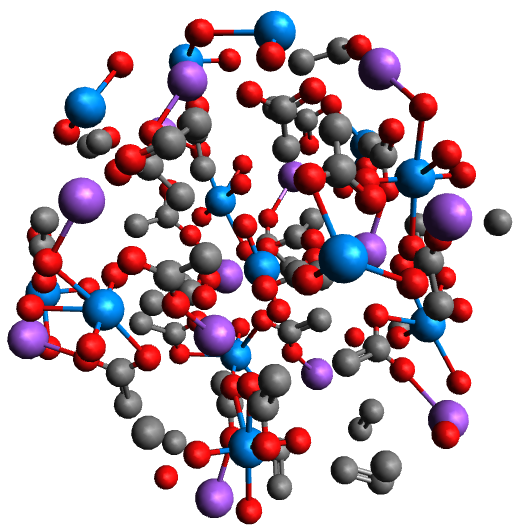
\includegraphics[width=\linewidth]{../ATEA/mfc/NaU_triacetate_full.png}

      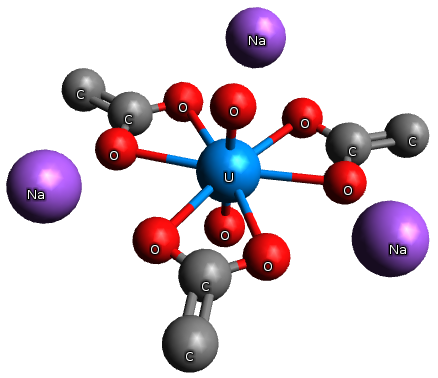
\includegraphics[width=\linewidth]{../ATEA/mfc/NaU_triacetate.png}
    \end{column}
  \end{columns}
\end{frame}

\defverbatim{\StyleElem}{%
\tiny
\begin{verbatim}
     0     92     U         
     1     92     U         
     2     11     Na        
     3     8      O         
     4     6      C
\end{verbatim}
\vspace{-3ex}
}
\defverbatim{\StyleSites}{%
\tiny
\begin{verbatim}
     0     92     U         
     1     92     U         
     2     11     Na        
     3     8      Oax         
     4     8      Oax         
     5     8      Oeq         
     6     8      Oeq         
     7     6      C
     8     6      C
\end{verbatim}
\vspace{-3ex}
}
\defverbatim{\StyleTags}{%
\tiny
\begin{verbatim}
     0     92     U
     1     92     U
     2     11     Na
     3     8      Oax
     4     8      Oeq
     5     6      C
\end{verbatim}
\vspace{-3ex}
}


\defverbatim[colored]{\AtomsListElem}{%
\tiny
\begin{alltt}
 {\color{SteelBlue4}ATOMS}
 {\color{Blue4}* x          y          z     ipot tag      distance}
  0.00000    0.00000    0.00000  0  U        0.00000
  1.01332    1.01332    1.01332  3  Oax.1    1.75512
 -1.01652   -1.01652   -1.01652  3  Oax.2    1.76067
  1.25061   -1.97853    0.76213  3  Oeq.1    2.46160
 -1.97853    0.76213    1.25061  3  Oeq.1    2.46160
  0.76213    1.25061   -1.97853  3  Oeq.1    2.46160
 -0.49169   -1.44195    1.94112  3  Oeq.2    2.46758
 -1.44195    1.94112   -0.49169  3  Oeq.2    2.46758
  1.94112   -0.49169   -1.44195  3  Oeq.2    2.46758
\end{alltt}
}

\defverbatim[colored]{\AtomsListSites}{%
\tiny
\begin{alltt}
 {\color{SteelBlue4}ATOMS}
 {\color{Blue4}* x          y          z     ipot tag      distance}
  0.00000    0.00000    0.00000  0  U        0.00000
  1.01332    1.01332    1.01332  4  Oax.1    1.75512
 -1.01652   -1.01652   -1.01652  3  Oax.2    1.76067
  1.25061   -1.97853    0.76213  6  Oeq.1    2.46160
 -1.97853    0.76213    1.25061  6  Oeq.1    2.46160
  0.76213    1.25061   -1.97853  6  Oeq.1    2.46160
 -0.49169   -1.44195    1.94112  5  Oeq.2    2.46758
 -1.44195    1.94112   -0.49169  5  Oeq.2    2.46758
  1.94112   -0.49169   -1.44195  5  Oeq.2    2.46758
\end{alltt}
}

\defverbatim[colored]{\AtomsListTags}{%
\tiny
\begin{alltt}
 {\color{SteelBlue4}ATOMS}
 {\color{Blue4}* x          y          z     ipot tag      distance}
  0.00000    0.00000    0.00000  0  U        0.00000
 {\color{DeepPink2} 1.01332    1.01332    1.01332  3  Oax.1    1.75512}
 {\color{DeepPink2}-1.01652   -1.01652   -1.01652  3  Oax.2    1.76067}
  1.25061   -1.97853    0.76213  4  Oeq.1    2.46160
 -1.97853    0.76213    1.25061  4  Oeq.1    2.46160
  0.76213    1.25061   -1.97853  4  Oeq.1    2.46160
 -0.49169   -1.44195    1.94112  4  Oeq.2    2.46758
 -1.44195    1.94112   -0.49169  4  Oeq.2    2.46758
  1.94112   -0.49169   -1.44195  4  Oeq.2    2.46758
\end{alltt}
}
  



\begin{frame}[fragile]
  \frametitle{Unique potentials in Feff}
  \begin{columns}[T]
    \begin{column}{0.5\linewidth}
      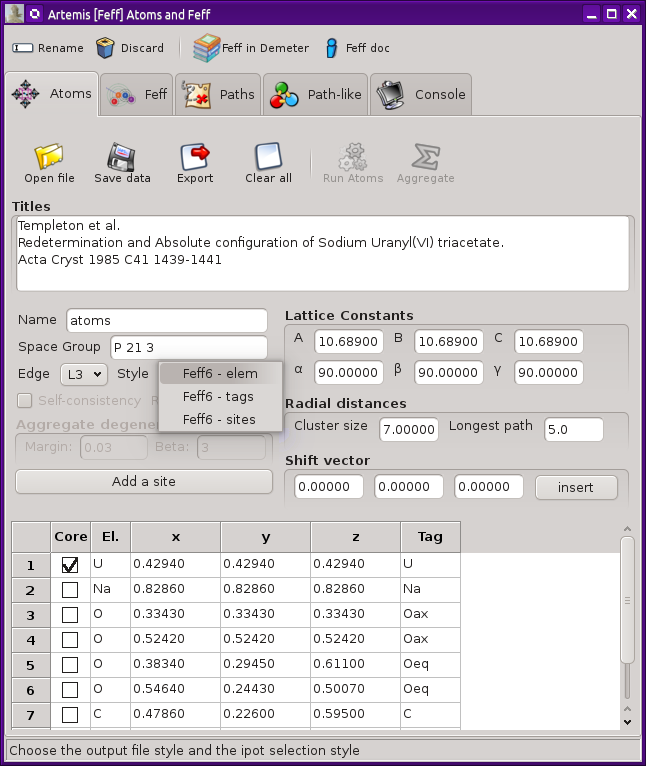
\includegraphics[width=0.9\linewidth]{images/atoms.png}
    \end{column}
    \begin{column}{0.5\linewidth}
      Style = \only<1>{elem}\only<2-3>{sites}\only<4>{tags}\\
      \vspace{-2ex}
      \begin{block}{}
        \tiny\begin{alltt}
 {\color{SteelBlue4}POTENTIALS}
  {\color{Blue4}* ipot   Z      tag}
        \end{alltt}
        \vspace{-9ex}
        \only<1>{\StyleElem}\only<2-3>{\StyleSites}\only<4>{\StyleTags}
      \end{block}
      \only<1>{
        \begin{exampleblock}{}
          \AtomsListElem
        \end{exampleblock}
      }
      \only<2>{
        \begin{exampleblock}{}
          \AtomsListSites
        \end{exampleblock}
      }
      \only<3>{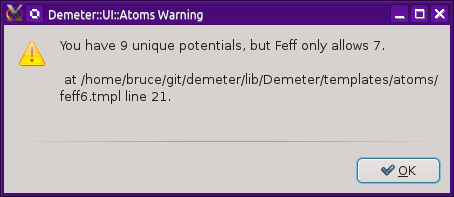
\includegraphics[width=\linewidth]{images/sites_error.png}}
      \only<4>{
        \begin{exampleblock}{}
          \AtomsListTags
        \end{exampleblock}
      }
    \end{column}
  \end{columns}
  \begin{block}<4>{}%
    Separate \texttt{ipot} values for the two O atoms allows
    \textsc{feff} to compute different muffin tin radii -- a good
    thing for the oxygenyl ligand.
  \end{block}
  \begin{textblock*}{0.33\linewidth}(12.0\TPHorizModule,10.3\TPVertModule)%
    \only<2>{
\includegraphics[width=\linewidth]{images/circle_x.png}}
  \end{textblock*}
\end{frame}

\begin{frame}
  \frametitle{The paths list}
  \begin{columns}[T]
    \begin{column}{0.5\linewidth}
      \begin{center}
        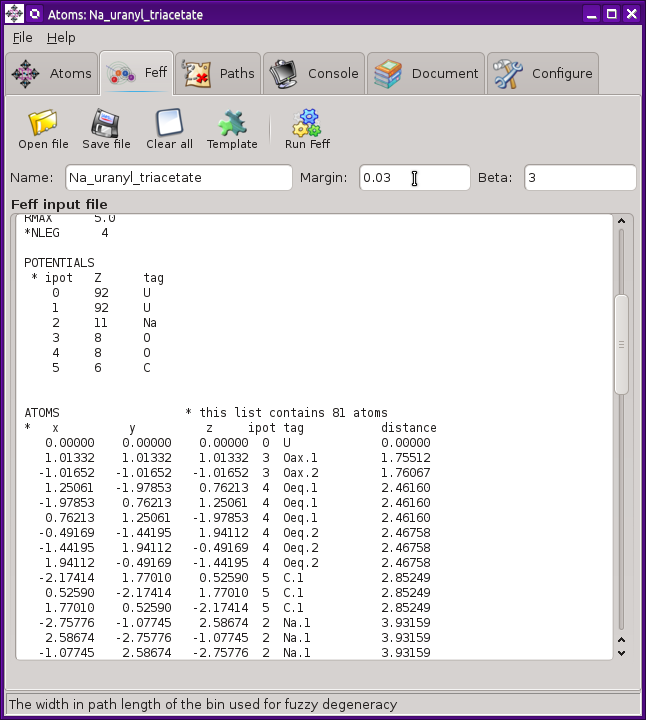
\includegraphics[width=0.85\linewidth]{images/feffinp.png}
      \end{center}
    \end{column}
    \begin{column}{0.5\linewidth}
      \begin{center}
        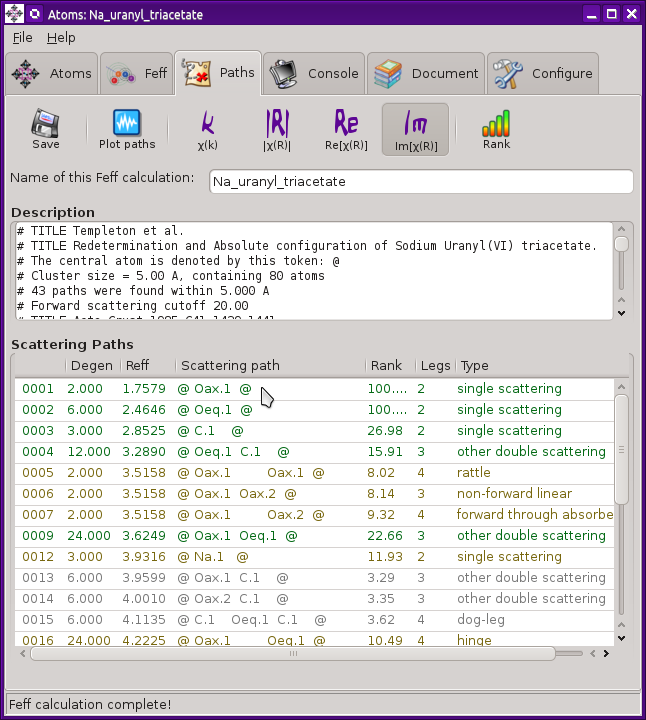
\includegraphics[width=0.85\linewidth]{images/paths.png}
      \end{center}
    \end{column}
  \end{columns}
  \begin{block}{Degeneracy margin}
    Fuzzy degeneracy ``collapses'' nearly degenerate paths, giving you
    fewer individual paths to worry about in the fit.
  \end{block}
\end{frame}

\begin{frame}
  \frametitle{Fit results}
  \begin{columns}[T]
    \begin{column}{0.5\linewidth}
      2 paths, 6 parameters -- pretty simple!

      \bigskip

      I get a very similar fit as the reference from GCA.

      \bigskip

      \begin{tabular}{lrr}
        \small parameter & GCA & Here \\
        \hline
        $S_0^2$         &   1.00(10) & 0.93(10) \\
        $R_{ax}$        &  1.80(1) & 1.78(1) \\
        $\sigma^2_{ax}$ &  0.001(1) & 0.002(1) \\
        $R_{eq}$        &  2.44(2) & 2.42(1) \\
        $\sigma^2_{eq}$ &  0.007(2) & 0.009(1) \\
      \end{tabular}
    \end{column}
    \begin{column}{0.5\linewidth}
      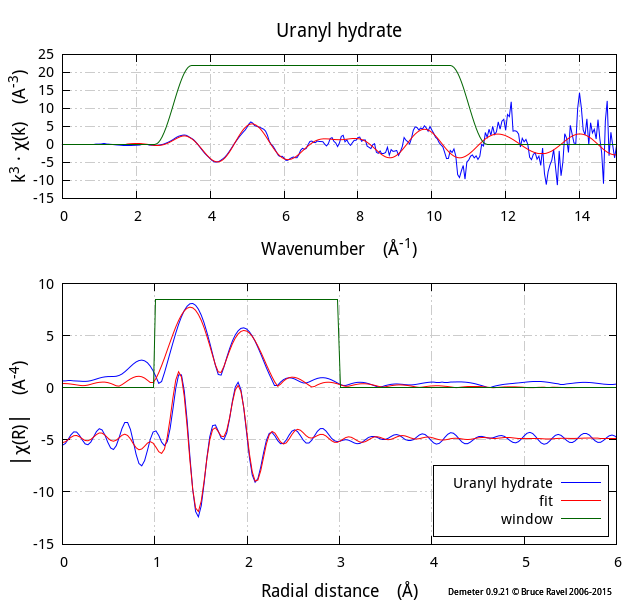
\includegraphics[width=0.85\linewidth]{images/fit.png}
    \end{column}
  \end{columns}
  \begin{textblock*}{0.7\linewidth}(0pt,19.0\TPVertModule)%
    \tiny%
    S.D.\ Kelly, et al., \textit{X-ray absorption fine structure
      determination of pH-dependent U-bacterial cell wall
      interactions}, Geochimica et Cosmochimica Acta \textbf{66}:22
    (2002) pp\  3855-3871.
    \href{http://dx.doi.org/10.1016/S0016-7037(02)00947-X}
    {\color{Blue4}\texttt{DOI:10.1016/S0016-7037(02)00947-X}}
  \end{textblock*}
\end{frame}

\begin{frame}
  \frametitle{So, is it data?}
  \begin{columns}
    \begin{column}{0.6\linewidth}
      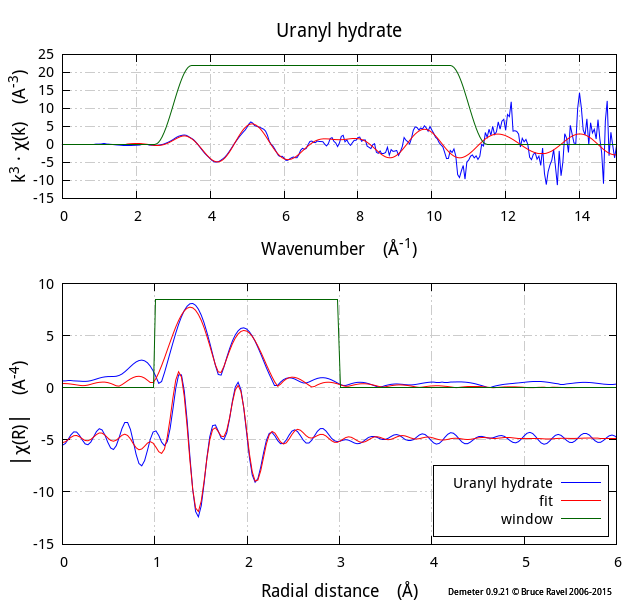
\includegraphics[width=0.85\linewidth]{images/fit.png}
    \end{column}
    \begin{column}{0.4\linewidth}
      There is clearly data beyond 9\,\AA$^{-1}$.

      \medskip

      In fact, I'd say there's data beyond 14\,\AA$^{-1}$!

      \medskip

      More measuring time would likely help in this case.
    \end{column}
  \end{columns}
\end{frame}

\end{document}

%%% Local Variables:
%%% mode: latex
%%% TeX-master: t
%%% TeX-parse-self: t
%%% TeX-auto-save: t
%%% TeX-auto-untabify: t
%%% TeX-PDF-mode: t
%%% End:
